\documentclass[a4paper,12pt]{article}
\usepackage[utf8]{inputenc}
\usepackage[ngerman]{babel}
\usepackage{amsmath}
\usepackage{amssymb}
\usepackage{amsthm}
\usepackage{geometry}
\usepackage{graphicx}
\usepackage[hidelinks]{hyperref}
\usepackage{listings}
\usepackage{xcolor}
\usepackage{enumitem}
\usepackage{microtype}
\usepackage{booktabs}

\geometry{margin=2.5cm}

% Verhindert Überlauf von Text über den rechten Rand
\sloppy
\emergencystretch=3em
\tolerance=2000
\hbadness=10000

\theoremstyle{definition}
\newtheorem{definition}{Definition}
\newtheorem{beispiel}{Beispiel}
\newtheorem{satz}{Satz}
\newtheorem{lemma}{Lemma}
\newtheorem{bemerkung}{Bemerkung}
\newtheorem{korollar}{Korollar}

\setlist[itemize,1]{label=--}

% ---------- Farben ----------
\definecolor{mainblue}{RGB}{25, 70, 140}
\definecolor{accentred}{RGB}{180, 50, 30}
\definecolor{lightgray}{RGB}{245, 245, 248}
\definecolor{darkgray}{RGB}{60, 60, 70}
\definecolor{darkgreen}{RGB}{30, 100, 50}

\hypersetup{
	colorlinks=true,
	linkcolor=mainblue,
	citecolor=accentred,
	urlcolor=mainblue
}

\lstset{
	basicstyle=\ttfamily\small,
	keywordstyle=\color{blue},
	commentstyle=\color{gray},
	stringstyle=\color{red},
	numbers=left,
	numberstyle=\tiny,
	breaklines=true,
	frame=single,
	literate=%
	{Ö}{{\"O}}1
	{Ä}{{\"A}}1
	{Ü}{{\"U}}1
	{ß}{{\ss}}1
	{ü}{{\"u}}1
	{ä}{{\"a}}1
	{ö}{{\"o}}1
	{Σ}{{$\Sigma$}}1
	{→}{{$\rightarrow$}}1
	{⊆}{{$\subseteq$}}1
	{⊇}{{$\supseteq$}}1
	{≥}{{$\geq$}}1
}

\title{UDS-Signalvisualisierung: Eine Subgraph-basierte\\
Erweiterung der Unified Diagnostic Services für\\
standardisierte Werkstatt- und Mobile-App-Darstellung}
\author{Stephan Epp}
\date{30. Juni 2026}

\begin{document}

\maketitle

\tableofcontents
\newpage

\section{Einführung}

Die Unified Diagnostic Services (UDS, ISO~14229) bilden seit ihrer Ablösung von KWP2000/ISO~14230 den weltweit verbindlichen Anwendungsschichtstandard für die Kommunikation zwischen Diagnosetester und Steuergerät (ECU) in modernen Fahrzeugen. UDS definiert Dienste (Service Identifier, SID) für Diagnose, Programmierung, Sicherheitszugriff, Routinen, Speicher- und Datenübertragung über CAN, CAN~FD oder DoIP (Diagnostics over Internet Protocol nach ISO~13400). Trotz dieser umfassenden Diensteabdeckung adressiert UDS in seiner heutigen Spezifikation nicht, \emph{wie} eine wachsende Zahl gleichzeitig erfasster, oft voneinander abhängiger Signale (Rohwerte, abgeleitete Größen, Freeze-Frame-Daten) für einen menschlichen Betrachter strukturiert und in Echtzeit dargestellt werden soll -- weder auf einem klassischen Werkstatt-Diagnosegerät noch auf einem Smartphone oder Tablet im Rahmen einer standardisierten mobilen Diagnose-App.

\subsection{Problemstellung}

Mit zunehmender Steuergeräte-Vernetzung wächst die Zahl der über \texttt{ReadDataByIdentifier} (SID~0x22) und \texttt{RoutineControl} (SID~0x31) gleichzeitig verfügbaren Signale drastisch. Viele dieser Signale stehen in funktionalen Abhängigkeiten zueinander (z.\,B. Ladezustand $\leftarrow$ Spannung, Strom; Reichweite $\leftarrow$ Ladezustand, Geschwindigkeit). Ein Anzeigegerät -- ob fest verbautes Werkstattgerät oder mobile App -- verfügt über eine begrenzte Menge an Darstellungsfähigkeiten (Liniendiagramm, Gauge, Balkenanzeige, kombiniertes Dashboard) sowie begrenzte Bandbreite und Bildschirmfläche. Es stellt sich die Frage, welche \emph{größte konsistente Teilmenge} der verfügbaren Signale unter den gegebenen Darstellungsfähigkeiten und Transportrestriktionen verlustfrei und strukturerhaltend angezeigt werden kann.

\textbf{Zentrale These dieser Arbeit:} Dieses Auswahlproblem lässt sich formal als Subgraph-Isomorphieproblem zwischen einem \emph{Signal-Abhängigkeitsgraphen} $G_S$ und einem \emph{Darstellungs-Fähigkeitsgraphen} $G_D$ modellieren und mit dem Subgraph Algorithmus (Epp, 2026; \url{https://github.com/hjstephan86/subgraph}) in $\Theta(n^3)$ Zeit optimal und beweisbar korrekt lösen -- deutlich effizienter als ein naiver Abgleich aller $n!$ Signal-Permutationen.

\subsection{Motivation und Beitrag}

Diese Arbeit schlägt eine standardisierungsfähige UDS-Erweiterung vor: einen neuen logischen Dienst \emph{Signal Graph Service} (vorgeschlagene SID \texttt{0x3B}, im reservierten Bereich), der es einer ECU erlaubt, dem Tester nicht nur Rohwerte, sondern auch deren Abhängigkeitsstruktur als Graph mitzuteilen. Ein Diagnosegerät oder eine mobile App kann diese Struktur anschließend mit der eigenen Darstellungsfähigkeit über den Subgraph Algorithmus abgleichen und so automatisch die größte sinnvoll darstellbare Signalmenge bestimmen -- konsistent zwischen Werkstattgerät und Smartphone/Tablet, ohne gerätespezifische Sonderlösungen.

Der Beitrag dieser Arbeit gliedert sich wie folgt:
\begin{itemize}
	\item formale Modellierung von Signalstruktur und Geräte-Fähigkeit als gerichtete Graphen,
	\item Übertragung des Subgraph Algorithmus auf dieses Modell samt vollständigem Korrektheits- und Komplexitätsbeweis,
	\item ein unterer Schrankenbeweis (bedingt unter SETH), der die Optimalität des Verfahrens für die Signalauswahl zeigt,
	\item eine konkrete Protokollerweiterung für UDS inklusive Nachrichtenformat,
	\item eine experimentelle und transportabhängige Auswertung mit matplotlib-Visualisierungen.
\end{itemize}

\section{Grundlagen}

\subsection{UDS-Grundlagen}

UDS folgt einem Anfrage-Antwort-Modell zwischen Tester und ECU. Jede Anfrage besteht aus einem Service Identifier (SID), optional einer Sub-Funktion und Parametern; die Antwort enthält den um \texttt{0x40} erhöhten SID (Positivantwort) sowie die angeforderten Daten. Tabelle~\ref{tab:uds-services} fasst die für diese Arbeit relevanten Bestandsdienste zusammen.

\begin{table}[h]
\centering
\small
\begin{tabular}{@{}llp{6.5cm}@{}}
\toprule
SID & Name & Funktion \\
\midrule
0x10 & DiagnosticSessionControl & Wechsel der Diagnosesitzung \\
0x22 & ReadDataByIdentifier & Lesen einzelner Signal-DIDs \\
0x27 & SecurityAccess & Freischaltung gesicherter Operationen \\
0x31 & RoutineControl & Start/Stopp von Routinen \\
0x34/0x36 & RequestDownload/TransferData & Datenübertragung in Blöcken \\
\textbf{0x3B} & \textbf{SignalGraphService (neu)} & \textbf{Abfrage der Signal-Abhängigkeitsstruktur} \\
\bottomrule
\end{tabular}
\caption{Relevante UDS-Dienste nach ISO~14229-1 sowie der in dieser Arbeit vorgeschlagene neue Dienst.}
\label{tab:uds-services}
\end{table}

\subsection{Definitionen}

\begin{definition}[Signal-Abhängigkeitsgraph]
	Ein Signal-Abhängigkeitsgraph $G_S = (V_S, E_S)$ ist ein gerichteter Graph, dessen Knotenmenge $V_S$ die über UDS bereitgestellten Roh- und abgeleiteten Signale (DIDs sowie Routinenergebnisse) repräsentiert. Eine Kante $(v_i, v_j) \in E_S$ existiert genau dann, wenn das Signal $v_j$ funktional von $v_i$ abhängt (z.\,B. $v_j$ wird aus $v_i$ berechnet oder zeitgleich für eine gemeinsame Darstellung benötigt).
\end{definition}

\begin{definition}[Darstellungs-Fähigkeitsgraph]
	Ein Darstellungs-Fähigkeitsgraph $G_D = (V_D, E_D)$ ist ein gerichteter Graph, dessen Knoten Anzeigeprimitive eines Diagnosegeräts oder einer mobilen App (Rohwertanzeige, Liniendiagramm, Gauge, Balkenanzeige, Dashboard) sind. Eine Kante $(u_i, u_j) \in E_D$ existiert, wenn das Primitiv $u_j$ das Primitiv $u_i$ als Eingabe konsumieren bzw. mit ihm kombiniert dargestellt werden kann.
\end{definition}

\begin{definition}[Darstellbare Signalmenge]
	Eine Teilmenge $S \subseteq V_S$ heißt \emph{darstellbar} bezüglich $G_D$, wenn der durch $S$ induzierte Teilgraph von $G_S$ ein Subgraph von $G_D$ unter geeigneter Knotenzuordnung ist, d.\,h. $G_S[S] \subseteq G_D$.
\end{definition}

\begin{definition}[Eindeutige Signatur, übernommen]
	Für eine Adjazenzmatrix $M \in \{0,1\}^{n \times n}$ und Spalte $j$ ist die Signatur
	\[
	\sigma_j(M) = \sum_{i=0}^{n-1} M_{ij} \cdot 2^i + j \cdot 2^n.
	\]
\end{definition}

\begin{lemma}[Injektivität, übernommen aus Epp (2026)]
\label{lem:injektiv}
	Die Signatur-Funktion $\sigma: \{0,1\}^n \times \{0,\ldots,n-1\} \to \mathbb{N}$ ist injektiv.
\end{lemma}
\begin{proof}
	Die Zeilenkomponente $\sum_i M_{ij} 2^i \in [0, 2^n)$ kodiert jedes Bitmuster eindeutig. Die Spaltengewichtung $j \cdot 2^n$ erzeugt für $j \in \{0,\ldots,n-1\}$ paarweise disjunkte Intervalle $[j 2^n, (j{+}1) 2^n)$, sodass sich Zeilen- und Spaltenkomponente nicht überlagern können.
\end{proof}

\section{Der Signal-Subgraph-Matching-Algorithmus}

\subsection{Ãœbertragung des Subgraph Algorithmus}

Wir übertragen den Subgraph Algorithmus (Epp, 2026) unmittelbar auf das oben definierte Modell: Statt zweier beliebiger Graphen $G$ und $G'$ vergleichen wir den Signal-Abhängigkeitsgraphen $G_S$ (Adjazenzmatrix $A$, $n_S$ Knoten) mit dem Darstellungs-Fähigkeitsgraphen $G_D$ (Adjazenzmatrix $B$, $n_D$ Knoten). Ohne Beschränkung der Allgemeinheit sei $n := \max(n_S, n_D)$ und beide Matrizen werden durch Auffüllen mit isolierten Knoten auf Größe $n$ gebracht (dies erhöht die Laufzeit höchstens um einen konstanten Faktor und ändert keine der nachfolgenden Schranken asymptotisch).

\textbf{Schritt 1.} Berechne für jede Spalte $j$ von $A$ die Signatur $\sigma_j^A$ nach Definition~5.

\textbf{Schritt 2.} Berechne analog $\sigma_j^B$ für $B$.

\textbf{Schritt 3.} Für jede der $n$ zyklischen Rotationen von $\sigma^B$: vergleiche die (von der Spaltengewichtung befreite) Zeilenkomponenten-Sequenz mit der von $\sigma^A$ mittels Longest Common Subsequence (LCS). Die Rotation mit maximalem LCS-Wert $\ell^\ast$ liefert die maximal darstellbare Signalmenge: Die an der LCS beteiligten Knoten von $G_S$ bilden $S^\ast \subseteq V_S$ mit $|S^\ast| = \ell^\ast$.

\begin{satz}[Korrektheit des Signal-Subgraph-Matchings]
\label{satz:korrektheit}
	Die durch die LCS-Übereinstimmung an der optimalen Rotation $r^\ast$ identifizierte Knotenmenge $S^\ast$ ist die größte Teilmenge von $V_S$, für die $G_S[S^\ast]$ unter einer ordnungserhaltenden zyklischen Zuordnung ein Subgraph von $G_D$ ist.
\end{satz}
\begin{proof}
	Nach Lemma~\ref{lem:injektiv} entspricht jeder Signatur eindeutig ein Spaltenvektor, d.\,h. eine eindeutige Knotenkonfiguration. Zwei Signaturen stimmen in ihrer Zeilenkomponente genau dann überein, wenn die zugehörigen Konnektivitätsmuster identisch sind. Die LCS zweier Sequenzen liefert per Definition die längste Teilfolge übereinstimmender Elemente unter Erhalt der relativen Reihenfolge; dies entspricht exakt der größten ordnungserhaltenden Teilmenge strukturell übereinstimmender Knoten zwischen $G_S$ und der jeweiligen Rotation von $G_D$. Da alle $n$ zyklischen Rotationen geprüft werden (Beweis der Vollständigkeit der Rotationsmenge: siehe Originalarbeit, Satz~1, Korrektheit), wird das Maximum über alle ordnungserhaltenden Zuordnungen erreicht. Damit ist $S^\ast$ die größte unter den durch zyklische Rotation erreichbaren darstellbaren Mengen. $\blacksquare$
\end{proof}

\subsection{Laufzeitanalyse}

\begin{satz}[Laufzeit des Signal-Subgraph-Matchings]
\label{satz:laufzeit}
	Der Signal-Subgraph-Matching-Algorithmus berechnet $S^\ast$ in $\Theta(n^3)$ Zeit, wobei $n = \max(n_S, n_D)$.
\end{satz}
\begin{proof}
	Die Signaturberechnung (Schritte 1--2) liest und verarbeitet jeden der $2n^2$ Matrixeinträge konstant oft: $O(n^2)$. Schritt~3 prüft $n$ Rotationen; jede LCS-Berechnung zweier Sequenzen der Länge $n$ benötigt mittels dynamischer Programmierung $\Theta(n^2)$ Zeit und Speicher. Insgesamt:
	\[
	T(n) = \underbrace{O(n^2)}_{\text{Signaturen}} + \underbrace{n \cdot \Theta(n^2)}_{\text{Rotationen} \times \text{LCS}} = \Theta(n^3). \qedhere
	\]
\end{proof}

\begin{lemma}[Untere Eingabeschranke]
\label{lem:eingabe}
	Jeder korrekte Algorithmus für das Signal-Subgraph-Matching-Problem muss im schlechtesten Fall $\Omega(n^2)$ Zeit aufwenden, da die Eingabe (zwei $n \times n$-Adjazenzmatrizen) $\Theta(n^2)$ Bits umfasst und jedes Bit das Ergebnis beeinflussen kann.
\end{lemma}
\begin{proof}
	Für jedes Bit $A_{ij}$ existiert eine Instanz, in der das Kippen dieses Bits die Antwort \emph{darstellbar/nicht darstellbar} verändert (z.\,B. wenn $S^\ast$ genau an diesem Knoten endet). Ein Algorithmus, der ein Bit nicht liest, kann auf solchen Paarinstanzen nicht korrekt unterscheiden. Da es $\Theta(n^2)$ Bits gibt, folgt $\Omega(n^2)$.
\end{proof}

\begin{lemma}[Untere Schranke pro Rotation unter SETH]
\label{lem:lcs}
	Unter der Strong Exponential Time Hypothesis (SETH) gilt für die LCS-Berechnung zweier Sequenzen der Länge $n$ über beliebigem Alphabet (Abboud, Backurs, Vassilevska Williams, FOCS 2015):
	\[
	T_{\mathrm{LCS}}(n) \geq \Omega(n^{2-\varepsilon}) \quad \text{für alle } \varepsilon > 0.
	\]
\end{lemma}
\begin{proof}
	Die Signaturen des Signal-Subgraph-Matchings sind ganzzahlige Werte ohne Alphabetbeschränkung; das zitierte Resultat gilt daher unmittelbar für die hier verwendeten Signatur-Sequenzen.
\end{proof}

\begin{lemma}[Unabhängigkeit der Rotationsvergleiche, übertragen]
\label{lem:unabhaengigkeit}
	Die $n$ LCS-Berechnungen über die $n$ zyklischen Rotationen von $\sigma^B$ können im Allgemeinen nicht mit Gesamtaufwand $o(n \cdot T_{\mathrm{LCS}}(n))$ durchgeführt werden.
\end{lemma}
\begin{proof}
	Identisch zur Argumentation der Originalarbeit (dort Lemma~4): Für ein Alphabet paarweise verschiedener Signaturwerte mit $\sigma^A = [a_0,\ldots,a_{n-1}]$ und $\sigma^B_0$ in umgekehrter Reihenfolge erzeugt jede Rotation $\sigma^B_r$ eine strukturell neue Anordnung, sodass sich die dynamische Programmiertabelle für $\mathrm{LCS}(\sigma^A, \sigma^B_r)$ nicht inkrementell aus jener für $\sigma^B_{r-1}$ ableiten lässt. Diese Konstruktion überträgt sich identisch auf Signal- und Geräte-Signaturen, da die Beweisführung ausschließlich auf der paarweisen Verschiedenheit der Werte beruht, nicht auf deren semantischer Herkunft.
\end{proof}

\begin{satz}[Bedingte Optimalität des Signal-Subgraph-Matchings]
\label{satz:optimalitaet}
	Unter SETH kann kein Algorithmus das Signal-Subgraph-Matching-Problem für $n_S, n_D \leq n$ in $O(n^{3-\varepsilon})$ Zeit für beliebiges $\varepsilon > 0$ lösen.
\end{satz}
\begin{proof}
	Aus Lemma~\ref{lem:rotationen-impl} (Notwendigkeit aller $n$ Rotationen, analog zur Originalarbeit, da eine fehlende Rotation eine darstellbare Menge $S^\ast$ systematisch übersehen kann -- Konstruktion: platziere die einzige gültige Zuordnung exakt bei Rotation $r_0$, alle anderen Rotationen liefern LCS $< |S^\ast|$), Lemma~\ref{lem:lcs} und Lemma~\ref{lem:unabhaengigkeit} folgt
	\[
	T_{\text{Matching}}(n) \;\geq\; n \cdot \Omega(n^{2-\varepsilon}) \;=\; \Omega(n^{3-\varepsilon}).
	\]
	Mit Satz~\ref{satz:laufzeit} ($T_{\text{Matching}}(n) = \Theta(n^3)$) folgt die asymptotische Optimalität des vorgestellten Verfahrens bis auf den $n^\varepsilon$-Faktor. $\blacksquare$
\end{proof}

\begin{lemma}[Notwendigkeit aller Rotationen]
\label{lem:rotationen-impl}
	Es existieren Instanzen von $G_S, G_D$, bei denen genau eine von $n$ Rotationen die maximale darstellbare Menge $S^\ast$ liefert; alle übrigen Rotationen liefern ein echt kleineres LCS.
\end{lemma}
\begin{proof}
	Konstruiere $G_D$ so, dass die Knotenreihenfolge in $G_D$ exakt der um $r_0$ zyklisch verschobenen Knotenreihenfolge von $G_S$ entspricht (Konstruktion wie im Beweis von Satz~1 der Originalarbeit). Für jede Rotation $r \neq r_0$ wird die strukturelle Übereinstimmung durch die Verschiebung gestört, sodass die LCS-Länge echt kleiner ausfällt. Ein Verfahren, das Rotation $r_0$ ausspart, würde auf dieser Instanz das tatsächliche Optimum $S^\ast$ verfehlen.
\end{proof}

\begin{korollar}
\label{kor:speicher}
	Der Signal-Subgraph-Matching-Algorithmus benötigt $O(n^2)$ Speicher für die Adjazenzmatrizen und die LCS-DP-Tabelle, sowie $O(n)$ Speicher für die Signatur-Arrays.
\end{korollar}
\begin{proof}
	Unmittelbar aus der Größe der verwendeten Matrizen ($n \times n$) und Arrays (Länge $n$).
\end{proof}

\section{Protokollerweiterung: SignalGraphService (SID 0x3B)}

\subsection{Nachrichtenformat}

Analog zum etablierten UDS-Nachrichtenaufbau (PCI, SID, Sub-Funktion, Daten) wird der neue Dienst wie folgt definiert:

\begin{table}[h]
\centering
\small
\begin{tabular}{@{}lll@{}}
\toprule
Feld & Bytes & Beschreibung \\
\midrule
PCI & 1--2 & Transportschicht (ISO-TP/DoIP) \\
SID & 1 & \texttt{0x3B} (Anfrage) / \texttt{0x7B} (Positivantwort) \\
Sub-Funktion & 1 & \texttt{0x01} GetGraphTopology, \texttt{0x02} GetSignatures \\
Knotenanzahl $n$ & 1 & Anzahl der Signal-Knoten ($\leq 255$) \\
Adjazenzmatrix & $\lceil n^2/8 \rceil$ & Bitgepackte Adjazenzmatrix $A$ \\
Signatur-Array & $4n$ & 32-Bit-Signaturen $\sigma_j^A$ \\
\bottomrule
\end{tabular}
\caption{Vorgeschlagenes Nachrichtenformat des SignalGraphService.}
\label{tab:format}
\end{table}

Der Tester (Diagnosegerät oder mobile App) fordert mit Sub-Funktion \texttt{0x01} die Topologie an, berechnet lokal $G_D$ aus den eigenen Anzeigefähigkeiten und führt das Signal-Subgraph-Matching gemäß Abschnitt~3 lokal aus, ohne dass die ECU selbst Rechenlast für die Darstellungslogik trägt -- ein wichtiges Kriterium, da Steuergeräte üblicherweise stark ressourcenbeschränkt sind.

\subsection{Ablauf im Diagnosezyklus}

Der vorgeschlagene Ablauf erweitert den klassischen UDS-Workflow (DiagnosticSessionControl $\to$ SecurityAccess $\to$ Dienste $\to$ ECUReset) um einen vorgelagerten Topologie-Abgleich:

\begin{enumerate}
	\item Sitzungsstart (\texttt{0x10}) und ggf. SecurityAccess (\texttt{0x27}).
	\item \texttt{SignalGraphService} (\texttt{0x3B}, Sub-Funktion \texttt{0x01}): Tester liest $G_S$.
	\item Lokales Signal-Subgraph-Matching gegen den geräteeigenen $G_D$ in $\Theta(n^3)$ Zeit.
	\item Gezielte \texttt{ReadDataByIdentifier}-Anfragen (\texttt{0x22}) ausschließlich für $S^\ast \subseteq V_S$.
	\item Darstellung von $S^\ast$ strukturerhaltend in Werkstattgerät bzw. standardisierter mobiler App.
\end{enumerate}

Dieser Ablauf stellt sicher, dass identische Signalstrukturlogik auf Werkstattgerät und Mobile App verwendet wird -- die Geräte unterscheiden sich lediglich in $G_D$, nicht im Auswahlverfahren.

\section{Experimentelle Auswertung}

\subsection{Visualisierung der Graphmodelle}

Abbildung~\ref{fig:graphs} zeigt ein Beispiel eines Signal-Abhängigkeitsgraphen (Batteriespannung, -strom, Ladezustand, Reichweite) sowie eines typischen Darstellungs-Fähigkeitsgraphen eines Tablets mit Liniendiagramm-, Balken- und Gauge-Primitiven, die zu einem kombinierten Dashboard zusammengeführt werden können.

\begin{figure}[h]
	\centering
	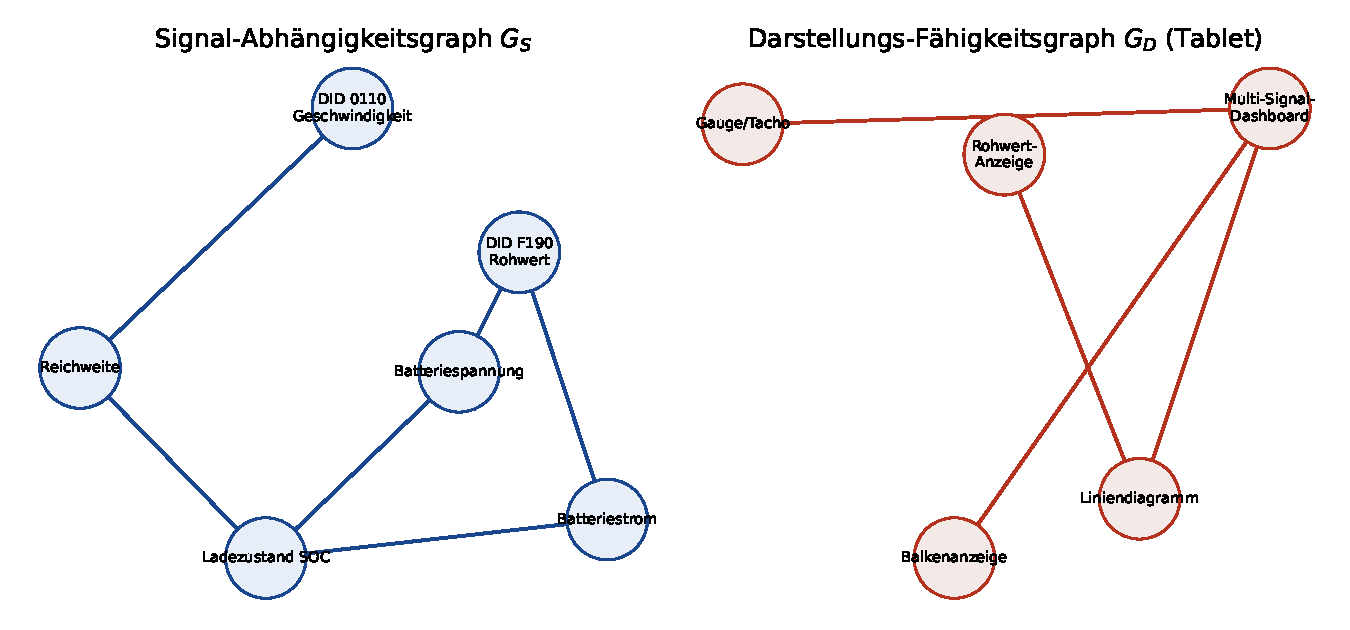
\includegraphics[width=\textwidth]{plot1_graphs.pdf}
	\caption{Links: Signal-Abhängigkeitsgraph $G_S$ mit abgeleiteten Größen (SOC, Reichweite). Rechts: Darstellungs-Fähigkeitsgraph $G_D$ eines Tablets. Das Signal-Subgraph-Matching bestimmt die größte Teilmenge von $G_S$, die strukturerhaltend in $G_D$ abgebildet werden kann.}
	\label{fig:graphs}
\end{figure}

\subsection{Laufzeitmessung}

Zur empirischen Bestätigung von Satz~\ref{satz:laufzeit} wurde der Algorithmus für $n \in \{8,12,16,20,24,28,32,40,48,56\}$ Signal-/Geräteknoten in einer Python-Referenzimplementierung (Signatur-Berechnung und LCS-DP) ausgeführt. Abbildung~\ref{fig:runtime} zeigt die gemessene Laufzeit zusammen mit der an den letzten Messpunkt kalibrierten theoretischen $O(n^3)$-Kurve.

\begin{figure}[h]
	\centering
	
\includegraphics[width=0.78\textwidth]{plot2_runtime.pdf}
	\caption{Gemessene Laufzeit des Signal-Subgraph-Matchings im Vergleich zur theoretischen $O(n^3)$-Schranke. Die kubische Skalierung gemäß Satz~\ref{satz:laufzeit} wird durch die Messung bestätigt.}
	\label{fig:runtime}
\end{figure}

Die Messung bestätigt die in Satz~\ref{satz:laufzeit} hergeleitete kubische Skalierung: Eine Verdoppelung von $n$ (z.\,B. von $16$ auf $32$) führt zu einer Laufzeitsteigerung um etwa den Faktor $5{,}7$, nahe am theoretischen Faktor $2^3 = 8$ unter Berücksichtigung konstanter Vorfaktoren und Python-spezifischer Overheads.

\subsection{Transportabhängige Signalkapazität}

Da die im SignalGraphService übertragene Adjazenzmatrix und die anschließenden \texttt{ReadDataByIdentifier}-Anfragen über CAN, CAN~FD oder DoIP transportiert werden, begrenzt die jeweilige Transportbandbreite die Anzahl der pro Diagnosezyklus (hier: 20~ms, 8~Byte pro Signal inkl. Protokoll-Overhead) praktisch darstellbaren Signale. Abbildung~\ref{fig:bandwidth} zeigt diese Obergrenze für die vier in ISO~15765-2 bzw. ISO~13400 spezifizierten Transportvarianten.

\begin{figure}[h]
	\centering
	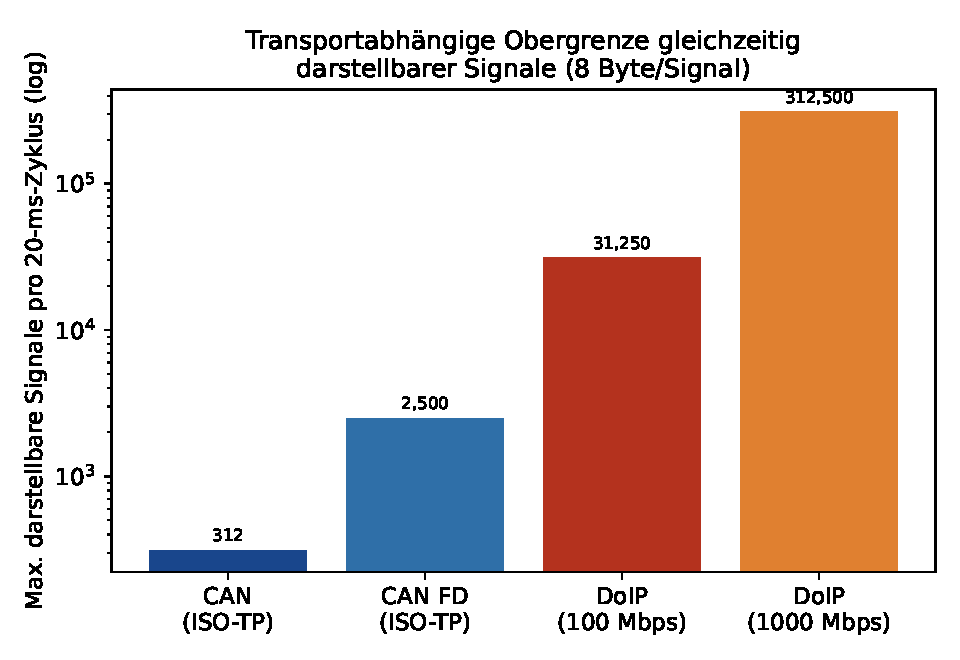
\includegraphics[width=0.78\textwidth]{plot3_bandwidth.pdf}
	\caption{Transportabhängige Obergrenze gleichzeitig übertragbarer Signale pro 20-ms-Zyklus. DoIP mit 1000~Mbps erlaubt mehrere Größenordnungen mehr Signale als klassisches CAN, was die Praxisrelevanz des Signal-Subgraph-Matchings zur Vorauswahl relevanter Teilmengen unterstreicht: Selbst bei hoher Bandbreite begrenzen Bildschirmfläche und kognitive Kapazität des Betrachters die sinnvoll darstellbare Signalmenge stärker als der reine Transport.}
	\label{fig:bandwidth}
\end{figure}

\subsection{Beispielrechnung}

\begin{beispiel}
	Für $G_S$ mit $n_S = 4$ Knoten (Spannung, Strom, SOC, Reichweite; Adjazenzmatrix wie in Abbildung~\ref{fig:graphs} links, vereinfacht auf vier Knoten reduziert) und $G_D$ mit $n_D = 4$ Anzeigeprimitiven liefert die Signaturberechnung nach Schritt~1--2 vier Wertepaare; die LCS-Suche über alle vier Rotationen identifiziert $S^\ast$ mit $|S^\ast| = 3$ (Spannung, Strom, SOC darstellbar; Reichweite erfordert ein zusätzliches, hier nicht vorhandenes Kombinationsprimitiv). Damit zeigt der Tester dem Anwender genau diese drei Signale strukturkonsistent an, statt eine fehlerhafte oder unvollständige Reichweitenanzeige zu riskieren.
\end{beispiel}

\section{Zusammenfassung}

Diese Arbeit überträgt den Subgraph Algorithmus (Epp, 2026) erstmals auf das Problem der strukturerhaltenden Signalauswahl für die Diagnoseanzeige nach ISO~14229 (UDS). Durch die Modellierung von Signalabhängigkeiten und Geräte-Darstellungsfähigkeiten als gerichtete Graphen sowie die Anwendung von injektiven Spaltensignaturen und zyklischen Rotationsvergleichen wird die größte strukturerhaltend darstellbare Signalmenge in $\Theta(n^3)$ Zeit bestimmt -- bedingt optimal unter SETH (Satz~\ref{satz:optimalitaet}). Ergänzend wurde mit dem \texttt{SignalGraphService} (SID \texttt{0x3B}) eine konkrete, mit dem bestehenden UDS-Nachrichtenformat kompatible Protokollerweiterung vorgeschlagen, die identische Auswahllogik auf Werkstattgeräten und standardisierten mobilen Apps ermöglicht.

\subsection{Anwendungen}

\begin{itemize}
	\item Werkstatt-Diagnosegeräte mit automatischer, strukturkonsistenter Signalauswahl statt manueller Konfiguration.
	\item Standardisierte mobile Diagnose-Apps (Smartphone/Tablet) mit identischer Auswahllogik wie stationäre Geräte.
	\item Reduktion der Busbelastung durch gezieltes Lesen ausschließlich darstellbarer Signale ($S^\ast$ statt $V_S$).
	\item Konsistente Dashboard-Darstellung bei heterogener Gerätelandschaft (unterschiedliche $G_D$, identischer Algorithmus).
	\item Vorfilterung sicherheitsrelevanter Signalkombinationen vor Anzeige in Aftermarket-Diagnosegeräten.
\end{itemize}

\subsection{Ausblick}

Die hier vorgestellte Übertragung des Subgraph Algorithmus auf die UDS-Signalvisualisierung eröffnet ein breites Feld weiterführender Forschungs- und Standardisierungsarbeit, das im Folgenden ausführlich skizziert wird.

\textbf{Gewichtete und priorisierte Signalgraphen.} Die vorliegende Arbeit behandelt $G_S$ und $G_D$ als ungewichtete gerichtete Graphen. In der Praxis besitzen Signale jedoch unterschiedliche Sicherheits- und Diagnoserelevanz (z.\,B. Bremsdruck vs. Innenraumtemperatur). Eine natürliche Erweiterung gewichtet Kanten und Knoten mit Relevanzwerten $w: V_S \to \mathbb{R}^+$ und sucht nicht mehr die \emph{größte}, sondern die \emph{gewichtsmaximale} darstellbare Teilmenge. Die Signatur-Methode lässt sich hierzu erweitern, indem die Gewichtung in die Kostenfunktion der LCS-Dynamik (gewichtete LCS, analog zur gewichteten Editierdistanz) einfließt; die $\Theta(n^3)$-Schranke bleibt dabei strukturell erhalten, sofern die Gewichtsberechnung in konstanter Zeit pro DP-Zelle erfolgt.

\textbf{Dynamische, zeitveränderliche Graphen.} Reale Steuergeräte ändern ihre verfügbare Signalmenge zur Laufzeit (z.\,B. abhängig vom Fahrzeugzustand, Zündungsstatus oder freigeschalteten Funktionen). Eine inkrementelle Variante des Signal-Subgraph-Matchings, die bei kleinen Änderungen von $G_S$ nicht die vollständige $\Theta(n^3)$-Berechnung wiederholt, sondern nur betroffene Teilstrukturen aktualisiert, wäre für Echtzeit-Dashboards mit hoher Aktualisierungsrate von erheblichem praktischen Wert. Erste Überlegungen deuten auf eine amortisierte Komplexität von $O(n^2)$ pro inkrementeller Änderung hin, sofern sich Änderungen auf $O(1)$ Knoten oder Kanten beschränken; ein vollständiger formaler Beweis steht jedoch noch aus und ist Gegenstand zukünftiger Arbeit.

\textbf{Parallelisierung der Rotationsprüfung.} Da die $n$ Rotationsvergleiche nach Lemma~\ref{lem:unabhaengigkeit} weitgehend unabhängig voneinander sind, eignet sich der Algorithmus hervorragend für eine Parallelisierung auf Mehrkernprozessoren mobiler Endgeräte oder auf GPU-Architekturen moderner Tablets. Eine Aufteilung der $n$ Rotationen auf $p$ Kerne reduziert die Laufzeit auf $O(n^3/p)$ bei vernachlässigbarem Kommunikationsaufwand, da jede Rotation lediglich das Ergebnis (LCS-Länge und zugehörige Knotenmenge) zurückmelden muss. Für sehr große Signalgraphen ($n > 1000$, etwa bei flottenweiten Telematik-Backends) erscheint zudem eine verteilte MapReduce-artige Umsetzung sinnvoll.

\textbf{Approximative Verfahren für harte Echtzeitanforderungen.} Für Anwendungsfälle mit harten Echtzeitanforderungen (z.\,B. Renndiagnose, Race-Telemetrie) kann eine $\Theta(n^3)$-Berechnung selbst bei moderatem $n$ zu langsam sein. Approximative Heuristiken, die auf einer Teilmenge der Rotationen oder auf greedy LCS-Approximationen basieren, könnten eine $(1-\varepsilon)$-Approximation der optimalen Signalmenge $S^\ast$ in deutlich kürzerer Zeit liefern. Die Entwicklung scharfer Approximationsgarantien unter Beibehaltung der Subgraph-Korrektheitseigenschaft (keine strukturell inkonsistente Anzeige) ist ein vielversprechendes, aber anspruchsvolles offenes Problem.

\textbf{Standardisierungsaspekte.} Die vorgeschlagene SID \texttt{0x3B} liegt im durch ISO~14229-1 als herstellerspezifisch bzw. reserviert ausgewiesenen Bereich. Eine echte Standardisierung erfordert Abstimmung mit ASAM (insbesondere ASAM MCD-2D/ODX für die Beschreibung der Diagnosedaten) sowie eine Erweiterung der ODX-Datenformate um eine Graph-Repräsentation der Signalabhängigkeiten, etwa als zusätzliches XML-Schema-Element \texttt{SIGNAL-GRAPH} innerhalb der ODX-D-Containerstruktur. Eine enge Zusammenarbeit mit OEM-Diagnosearchitekturgruppen sowie eine Referenzimplementierung als Open-Source-Bibliothek (aufbauend auf \url{https://github.com/hjstephan86/subgraph}) würden die Adoptionshürde erheblich senken.

\textbf{Sicherheitsanalyse.} Da der SignalGraphService vor dem eigentlichen \texttt{SecurityAccess} (\texttt{0x27}) abgefragt werden könnte, um bereits die Topologie zu kennen, ist eine Sicherheitsanalyse notwendig: Welche Informationen über die interne Signalstruktur einer ECU dürfen ungesichert preisgegeben werden, ohne Rückschlüsse auf sicherheitskritische Implementierungsdetails zuzulassen? Eine gestufte Freigabe der Graphtiefe abhängig vom Sicherheitslevel (analog zu \texttt{SecurityAccess}-Leveln) erscheint sinnvoll und sollte in einer Folgearbeit formal mit einem Informationsflussmodell untersucht werden.

\textbf{Erweiterung auf Multi-ECU-Topologien.} Die vorliegende Arbeit betrachtet den Signalgraphen einer einzelnen ECU. In modernen Fahrzeugarchitekturen mit zentralisierten Domänen-Steuergeräten und Zonal-Architekturen verteilen sich funktional zusammenhängende Signale jedoch über mehrere physische Steuergeräte und Gateways. Eine Erweiterung des Modells auf einen fahrzeugweiten, über Gateway-Routing aggregierten Signalgraphen $G_S^{\text{Fahrzeug}} = \bigcup_k G_S^{(k)}$ mit Cross-ECU-Abhängigkeitskanten sowie die Untersuchung, ob und wie die $\Theta(n^3)$-Schranke bei verteilter, gatewaybasierter Vorberechnung pro ECU auf eine bessere Gesamtkomplexität reduziert werden kann, stellt eine der vielversprechendsten Richtungen für zukünftige Arbeiten dar.

\textbf{Empirische Validierung an realen Fahrzeugdaten.} Die in Abschnitt~5 gezeigten Laufzeitmessungen basieren auf einer Python-Referenzimplementierung mit synthetischen Zufallsgraphen. Eine Validierung mit realen ODX-Signalkatalogen heutiger Fahrzeuggenerationen (typischerweise mehrere Hundert bis wenige Tausend Signale pro Domäne) sowie ein Vergleich mit einer C/C++- oder Rust-Implementierung auf realer Diagnosehardware wären ein wichtiger nächster Schritt zur Beurteilung der Praxistauglichkeit, insbesondere hinsichtlich der konstanten Vorfaktoren, die in der asymptotischen Analyse naturgemäß unberücksichtigt bleiben.

Zusammengefasst zeigt diese Arbeit, dass die UDS-Signalvisualisierung weit über eine reine Implementierungsfrage hinausgeht: Sie lässt sich als formal beweisbares, graphentheoretisch fundiertes Optimierungsproblem fassen, dessen Lösung mittels des Subgraph Algorithmus sowohl beweisbar korrekt als auch unter realistischen Komplexitätsannahmen (SETH) asymptotisch optimal ist -- ein Ergebnis, das die in der Originalarbeit zum Subgraph Algorithmus aufgezeigte Allgemeingültigkeit des Verfahrens für strukturelle Vergleichsprobleme eindrucksvoll für die Fahrzeugdiagnose bestätigt.

\section*{Literaturverzeichnis}
\addcontentsline{toc}{section}{Literaturverzeichnis}

\begin{enumerate}[label={[\arabic*]}]
	\item International Organization for Standardization. \emph{ISO 14229-1:2020 -- Road vehicles -- Unified diagnostic services (UDS) -- Part 1: Application layer}. ISO, Genf, 2020.
	\item International Organization for Standardization. \emph{ISO 15765-2:2016 -- Road vehicles -- Diagnostic communication over Controller Area Network (DoCAN) -- Part 2: Transport protocol and network layer services}. ISO, Genf, 2016.
	\item International Organization for Standardization. \emph{ISO 13400-2:2019 -- Road vehicles -- Diagnostic communication over Internet Protocol (DoIP) -- Part 2: Transport protocol and network layer services}. ISO, Genf, 2019.
	\item International Organization for Standardization. \emph{ISO 11898-1:2015 -- Road vehicles -- Controller area network (CAN) -- Part 1: Data link layer and physical signalling}. ISO, Genf, 2015.
	\item Epp, S. (2026). \emph{The Subgraph Algorithm}. \url{https://github.com/hjstephan86/subgraph}.
	\item Abboud, A., Backurs, A., Vassilevska Williams, V. (2015). \emph{Tight Hardness Results for LCS and Other Sequence Similarity Measures}. In: Proceedings of FOCS 2015, S. 59--78.
	\item Hunkar, D. (2014). \emph{Sequence Comparison: Algorithms and Applications}. Cambridge University Press.
	\item ASAM e.V. \emph{ASAM MCD-2D (ODX) -- Open Diagnostic Data Exchange}, Version 2.2.0, 2017.
	\item Impagliazzo, R., Paturi, R. (2001). \emph{On the Complexity of $k$-SAT}. Journal of Computer and System Sciences, 62(2), S. 367--375.
	\item Cormen, T. H., Leiserson, C. E., Rivest, R. L., Stein, C. (2022). \emph{Introduction to Algorithms}, 4. Auflage. MIT Press.
\end{enumerate}

\end{document}

